%================================================================
\section{Results and Discussion}\label{sec:Results}
%================================================================

%----------------------------------------------------------------
\subsection{Project Results 1}\label{sec:project results}
%----------------------------------------------------------------

%----------------------------------------------------------------
\subsection{Heat Equation}\label{sec:heateq results}
%----------------------------------------------------------------



\subsubsection{FFNN}


%----------------------------------------------------------------
\subsection{Eigenvalue Problem}\label{sec:eigenvalue results}
%----------------------------------------------------------------

Accompanying notebook: 


\subsubsection*{Benchmark ODE rhs with Euler}

\autoref{fig:euler_benchmark}, ODE RHS, two alternatives, benchmark which gives best result with Euler's method. simulation, time $t\in [0, 5]$ with $N = 101$ number of timesteps

\begin{figure}[H]
\centering
\subfloat[]{{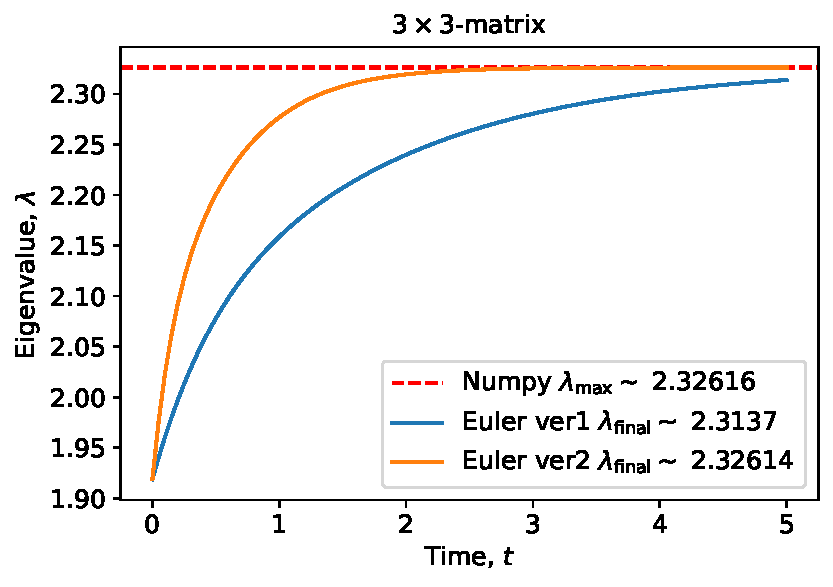
\includegraphics[scale=0.5]{latex/figures/euler_benchmark_33.pdf}}}
\qquad
\subfloat[]{{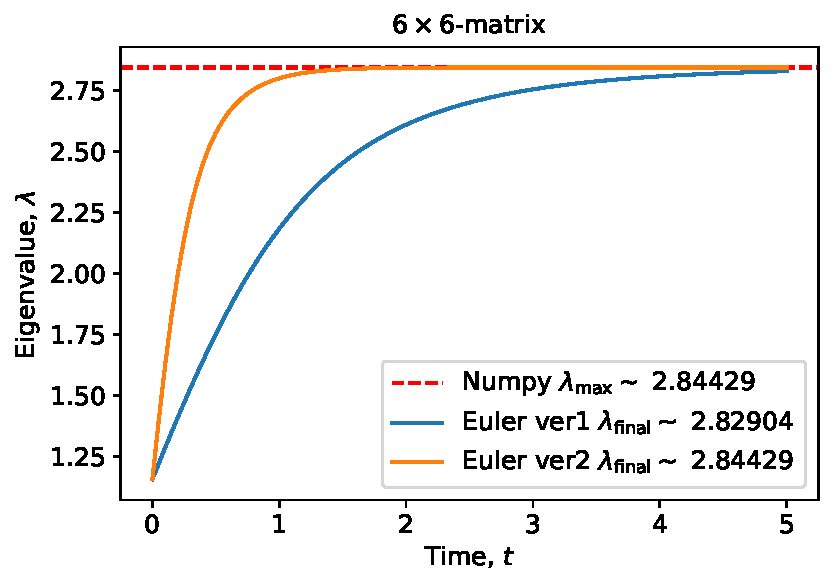
\includegraphics[scale=0.5]{latex/figures/euler_benchmark_66.pdf}}}
\caption{Euler's method with different expressions of the right-hand side of ODE (ref) tested on randomly generated real symmetric matrices; in \textbf{(a)} a $3\times 3$-matrix, and in \textbf{(b)} a $6\times 6$-matrix.}
\label{fig:euler_benchmark}
\end{figure}

From the figures it seems like ODE RHS ver1 converges somewhat slower than ver2 in the 3x3 case. In the 6x6 case, however, ver1 often struggles to converge as good as ver2 (multiple runs, which can be easily reproduced in jupyter notebook). Both these 'problems' probably arises because ver1 is more computationally demanding than ver2.

\subsubsection{FFNN, benchmark problem}

\begin{equation*}
    A = \left(\begin{array}{ccc}
        3 & 2 & 4  \\
        2 & 0 & 2  \\
        4 & 2 & 3
    \end{array}\right)
\end{equation*}
with eigenvalues $\lambda_1 = 8$ and $\lambda_2 = \lambda_3 = -1$.



\autoref{fig:benchrun1}; 3 layers + output [sigmoid, relu, sigmoid], [100, 50, 25]

Step: 1500, Loss: 0.014227586970184775

A = [[3. 2. 4.]
 [2. 0. 2.]
 [4. 2. 3.]]
x0 = [1 0 0]
Eigvals Numpy: [-1.  8. -1.]
Max Eigval Numpy 8.0
Final Eigval Euler 7.999999884131663
Final Eigval FFNN 7.999994245949094

\begin{figure}[H]
\centering
\subfloat[]{{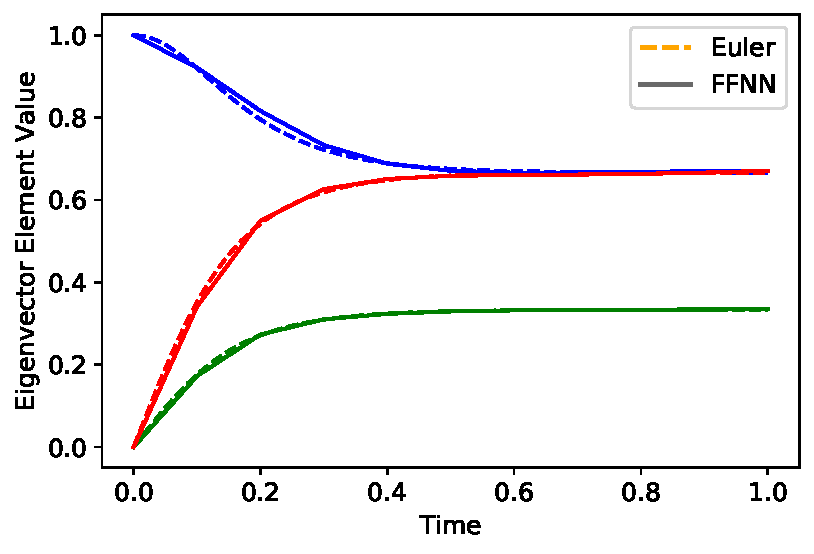
\includegraphics[scale=0.5]{latex/figures/eigvec_comp_benchrun1.pdf}}}
\qquad
\subfloat[]{{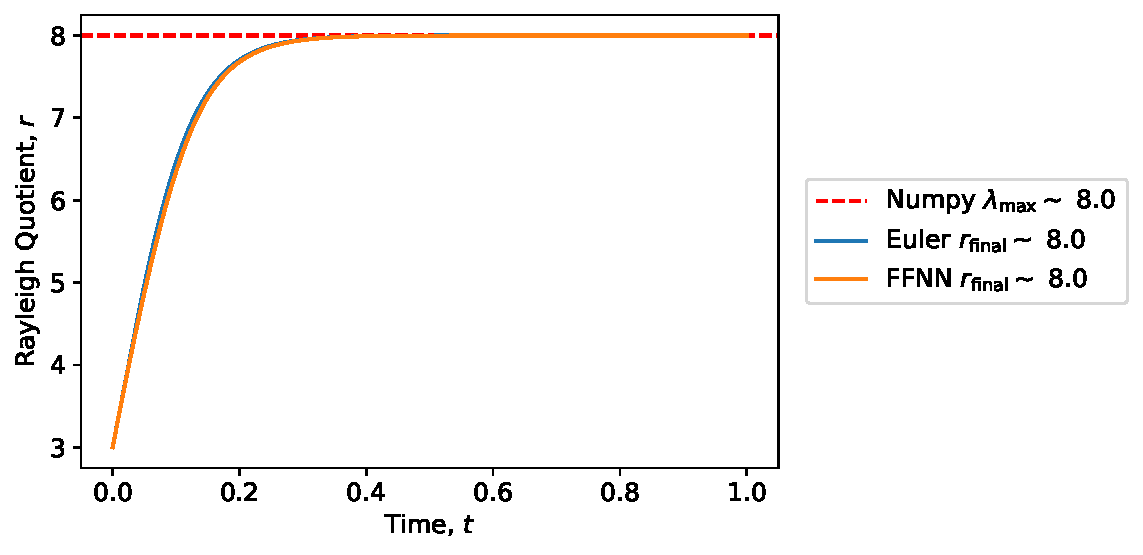
\includegraphics[scale=0.5]{latex/figures/eigval_benchrun1.pdf}}}
\caption{Benchrun 1 \textbf{(a)} Components of steady-state vector computed with both Euler's method (dashed lines) and the feed-forward neural network (solid line). \textbf{(b)} Computed maximum eigenvalue }
\label{fig:benchrun1}
\end{figure}

